\documentclass{article}\usepackage[]{graphicx}\usepackage[]{color}
%% maxwidth is the original width if it is less than linewidth
%% otherwise use linewidth (to make sure the graphics do not exceed the margin)
\makeatletter
\def\maxwidth{ %
  \ifdim\Gin@nat@width>\linewidth
    \linewidth
  \else
    \Gin@nat@width
  \fi
}
\makeatother

\definecolor{fgcolor}{rgb}{0.345, 0.345, 0.345}
\newcommand{\hlnum}[1]{\textcolor[rgb]{0.686,0.059,0.569}{#1}}%
\newcommand{\hlstr}[1]{\textcolor[rgb]{0.192,0.494,0.8}{#1}}%
\newcommand{\hlcom}[1]{\textcolor[rgb]{0.678,0.584,0.686}{\textit{#1}}}%
\newcommand{\hlopt}[1]{\textcolor[rgb]{0,0,0}{#1}}%
\newcommand{\hlstd}[1]{\textcolor[rgb]{0.345,0.345,0.345}{#1}}%
\newcommand{\hlkwa}[1]{\textcolor[rgb]{0.161,0.373,0.58}{\textbf{#1}}}%
\newcommand{\hlkwb}[1]{\textcolor[rgb]{0.69,0.353,0.396}{#1}}%
\newcommand{\hlkwc}[1]{\textcolor[rgb]{0.333,0.667,0.333}{#1}}%
\newcommand{\hlkwd}[1]{\textcolor[rgb]{0.737,0.353,0.396}{\textbf{#1}}}%

\usepackage{framed}
\makeatletter
\newenvironment{kframe}{%
 \def\at@end@of@kframe{}%
 \ifinner\ifhmode%
  \def\at@end@of@kframe{\end{minipage}}%
  \begin{minipage}{\columnwidth}%
 \fi\fi%
 \def\FrameCommand##1{\hskip\@totalleftmargin \hskip-\fboxsep
 \colorbox{shadecolor}{##1}\hskip-\fboxsep
     % There is no \\@totalrightmargin, so:
     \hskip-\linewidth \hskip-\@totalleftmargin \hskip\columnwidth}%
 \MakeFramed {\advance\hsize-\width
   \@totalleftmargin\z@ \linewidth\hsize
   \@setminipage}}%
 {\par\unskip\endMakeFramed%
 \at@end@of@kframe}
\makeatother

\definecolor{shadecolor}{rgb}{.97, .97, .97}
\definecolor{messagecolor}{rgb}{0, 0, 0}
\definecolor{warningcolor}{rgb}{1, 0, 1}
\definecolor{errorcolor}{rgb}{1, 0, 0}
\newenvironment{knitrout}{}{} % an empty environment to be redefined in TeX

\usepackage{alltt}

% Packages and Settings for LaTeX
\input{"C:/Users/Beniamino/Desktop/Mini_Project_1/Code/definitions"}


\title{\textbf{Dynamic Harmonic Regression}}
\author{Beniamino Hadj-Amar}
\IfFileExists{upquote.sty}{\usepackage{upquote}}{}
\begin{document}

\maketitle

\renewenvironment{knitrout}{\vspace{1em}}{\vspace{1em}}



\begin{tcolorbox}

\textbf{Observation Equation}: $ y_t = H_t x_t + e_t $
\\\textbf{State Equation}: $ \qquad \quad \, \,   x_t = F x_{t-1} + G \eta_t $

\end{tcolorbox}

where $e_t \sim \mathcal{N}(0, \sigma^2)$ and $\eta_t \sim \mathcal{N}(0, Q)$

\section*{Estimation of the time variable parameters}

Suppose $x_{t-1}| y^{t-1} \sim \mathcal{N}(x_{t-1} | \hat{x}_{t-1}, P_{t-1}) $

\subsection*{1 - Forward Pass Filtering Equations}
\subsubsection*{\underline{Prediction}}

$ \hat{x}_{t|t-1} = \mathbb{E} [ x_t | y^{t-1} ] =  F \hat{x}_{t-1} $

$ P_{t| t-1} = \mathbb{V}\text{ar}[x_t | y^{t-1} ] = F P_{t-1} F^T + G Q_r G^T $

\subsubsection*{\underline{Correction}}

$ \hat{x}_t = \mathbb{E} [x_t | y^t] = \hat{x}_{t|t-1} + P_{t| t-1} H_t^T \Big[ 1 + H_t P_{t| t-1} H_t^T \Big]^{-1}  \{ y_t - H_t \hat{x}_{t|t-1}  \} $

$ P_t = \mathbb{V}ar [x_t | y^t] = P_{t | t-1} - P_{t | t-1} H_t^T \Big[ 1 + H_t P_{t| t-1} H_t^T \Big]^{-1} H_t P_{t | t-1} $



\subsection*{Backward Pass Smoothing Equations}

$\hat{x}_{t | N} = F^{-1} \Big[ \hat{x}_{t+1 | N} + G Q_r G^T L_t \Big]$

$L_t = \Big[ I - P_{t+1} H_{t+1}^T H_{t+1} \Big]^{T} \Big[ F^T L_{t+1} - H_{t+1}^T \{y_{t+1} - H_{t+1}\hat{x}_{t+1} \} \Big]  $

$P_{t|N} = P_t + P_t F^T P_{t+1|t}^{-1} \Big[ P_{t+1|N} - P_{t+1 | t} \Big] P_{t+1 | t}^{-1} F P_t $

\vspace{0.2cm}
where $Q_r$ = $\dfrac{Q}{\sigma^2}$, and $P_t = \dfrac{P_t^{*}}{\sigma^2}. \quad $ $P_t^{*}$ is the error covariance matrix associated with the state estimates.





\newpage

\section*{Spectral Analysis of DHR model}

\subsection*{IRW}

Consider UC model, consisting only of an \textbf{IRW} trend plus a white noise component: 


\begin{align} \label{eqIRW}
x_t &=  x_{t-1} +  \nabla x_{t-1}  \\ 
\nabla x_{t} &= \nabla x_{t-1} + \eta_{t-1} \\
y_t &= x_t + {e_t}
\end{align}

By plugging (2) in (1) we obtain:

\begin{equation*}
\begin{split}
x_t &= x_{t-1} + \nabla x_{t-2} + \eta_{t-1} \\
x_t   & =   x_{t-1} + x_{t-1} - x_{t-2} + \eta_{t-1} \\
x_t - 2 x_{t-1} + x_{t-2} &= \eta_{t-1} \\
(1 - L)^2 x_t &= \eta_{t-1} \\
x_t &= \frac{1}{(1 - L)^2} \eta_{t-1}
\end{split}
\end{equation*}

Therefore, the observational equation can be written as

\begin{equation*}
\boxed{
y_t = x_t + e_t = \frac{1}{(1 - L)^2} \eta_{t-1} + {e_t}
}
\end{equation*}

where L is the backward shift operator. 

We take the second differences of $y_t$ in order to capture the non stationarity of the IRW process:

\begin{equation*}
\nabla^2 y_t = \eta_{t-1} + \nabla^2 e_t, \quad \text{where} \quad \nabla = (1 -L).
\end{equation*}

In order to evaluate the power spectrum of the process $\nabla^2 y_t$ we need to compute its covariance function:



\begin{equation*}
\gamma_{\nabla^2 y}(h)  = \gamma_{\eta}(h) + \gamma_{\nabla^2 e}(h)
\end{equation*}

Hence,


\[ 
\gamma_{\nabla^2 y}(h) = 
  \begin{cases}
  \sigma^2_{\eta} + 6 \sigma^2 & \text{if } h = 0 \\
  \quad -4 \sigma^2                  & \text{if } |h| = 1 \\
  \quad \sigma^2                     & \text{if } |h| = 2 \\
  \quad 0                            & \text{if } |h| > 2
  \end{cases}
\]


Therefore, the \textbf{power frequency spectrum} is given by:

\begin{equation} \label{spectrum}
\begin{split}
f_{\nabla^2 y}(\omega) & = \frac{1}{2 \pi} \sum_{h \in \mathbb{Z}} \gamma_{\nabla^2 y}(h) \cdot \text{exp}\{-i2\pi\omega h\} \\
 & = \frac{1}{2\pi} \Big[  \sigma^2_{\eta} + 6\sigma^2 - 8\sigma^2 \text{cos}(\omega) + 2\sigma^2 \text{cos}(2\omega) \Big] \\
 & = \frac{1}{2\pi} \Big[ \sigma^2_{\eta} + \sigma^2 \{ 2 - 2\text{cos}(\omega)\}^2 \Big].
\end{split}
\end{equation}
In order to compute \eqref{spectrum} we used the following identities: 

\textbf{-} $2\text{cos}(\omega) = \text{exp}(i\omega) +  \text{exp}(-i\omega) $

\textbf{-} $\text{cos}(2\omega) = \text{cos}^2(\omega) - 1 $

\vspace{0.3cm}

The pseudo-spectrum of IRW is given by



\begin{equation*}
f_y(\omega) = \dfrac{1}{2\pi} \Big[ \dfrac{\sigma^2_{\eta}}{\{2-2\text{cos}(\omega)\}^2} + \sigma^2\Big]
\end{equation*}



\subsection*{RW}
Consider UC model, with a RW trend plus a with noise component:

\begin{equation*}
\begin{split}
x_t &= x_{t-1} + \eta_{t-1} \\
y_t &= x_t + {e_t}
\end{split}
\end{equation*}

Hence, the observational equation can be written as

\begin{equation*}
\boxed{
y_t = \dfrac{1}{1-L}\eta_{t-1} + {e_t}
}
\end{equation*}

We can look at the first differences to study the inhernet non stationarity of the process:

\begin{equation*}
\nabla y_t = \eta_{t-1} + \nabla{e_t}
\end{equation*}

The pseudo-spectrum in the case of the RW trend is given by

\begin{equation*}
f_y(\omega) = \dfrac{1}{2\pi} \Big[ \dfrac{\sigma^2_{\eta}}{\{2-2\text{cos}(\omega)\}} + \sigma^2\Big]
\end{equation*}

\newpage

The code to evaluate the IRW and RW pseudo-spectrum is given by:

\begin{knitrout}\footnotesize
\definecolor{shadecolor}{rgb}{0.969, 0.969, 0.969}\color{fgcolor}\begin{kframe}
\begin{alltt}
\hlcom{# Pseudo-Spectrum Generalised Random Walk (GRW)}
\hlstd{pseudo.spectrum.GRW} \hlkwb{<-} \hlkwa{function}\hlstd{(}\hlkwc{omega}\hlstd{,} \hlkwc{sigma2.eta}\hlstd{,} \hlkwc{sigma2}\hlstd{,}
                                \hlkwc{type} \hlstd{=} \hlstr{"IRW"}\hlstd{,} \hlkwc{alpha} \hlstd{=} \hlnum{1}\hlstd{) \{}
  \hlkwa{if}\hlstd{(type} \hlopt{==} \hlstr{"IRW"}\hlstd{) \{}
    \hlstd{alpha} \hlkwb{<-} \hlnum{1}
  \hlstd{\}}
  \hlkwa{else if}\hlstd{(type} \hlopt{==} \hlstr{"RW"}\hlstd{) \{}
    \hlstd{alpha} \hlkwb{<-} \hlnum{0}
  \hlstd{\}}

  \hlstd{spectrum} \hlkwb{<-} \hlstd{(}\hlnum{1}\hlopt{/}\hlstd{(}\hlnum{2}\hlopt{*}\hlstd{pi))} \hlopt{*} \hlstd{(  (sigma2.eta}\hlopt{/}\hlstd{((}\hlnum{1} \hlopt{+} \hlstd{(alpha}\hlopt{^}\hlnum{2}\hlstd{)} \hlopt{-} \hlstd{(}\hlnum{2}\hlopt{*}\hlstd{alpha}\hlopt{*}\hlkwd{cos}\hlstd{(omega)) )} \hlopt{*}
                                             \hlstd{(}\hlnum{2} \hlopt{-} \hlnum{2}\hlopt{*}\hlkwd{cos}\hlstd{(omega))))} \hlopt{+} \hlstd{sigma2   )}
  \hlkwd{return}\hlstd{(spectrum)}
\hlstd{\}}
\end{alltt}
\end{kframe}
\end{knitrout}


We show in \ref{fig:ciao} properties of the pseudo spectra of RW and IRW process, for different value of NVR $\dfrac{\sigma^2_{\eta}}{\sigma^2}$:

\begin{figure}[htbp]
\centering
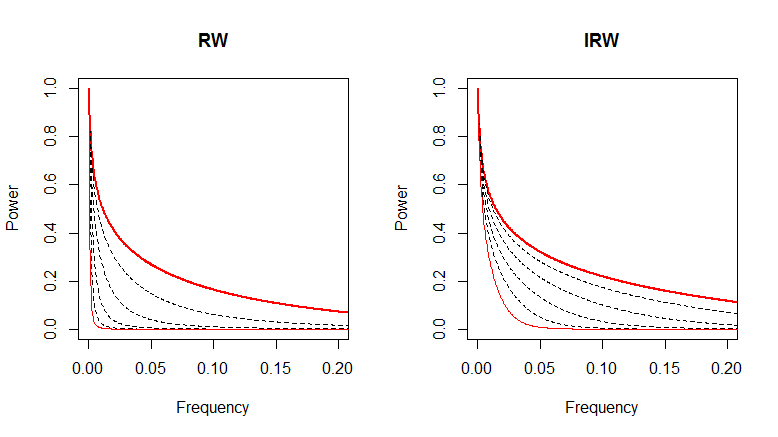
\includegraphics[scale = 0.5]{Plots/RWvsIRW.png}
\caption{Pseudo-Spectrum RW and IRW: thick red line is for value of NVR of $10^{-1}$; thin red line is for value of NVR of $10^{-6}$. Also, we took the log of the spectrum, and normalise it to the range [0, 1]}
\label{fig:ciao}
\end{figure}

\newpage

\subsection*{Pseudo-spectra of the Full DHR Model}

If we consider a single frequency $\omega_j$ DHR term of the form $S_t = a_t \text{cos}(\omega_j t) + b_t \text{sin}(\omega_j t) $, where $a_t$ and $b_t$ follow an IRW or RW process with equal variance parameters $\sigma^2_{\omega_j}$

The pseudo spectrum for the IRW and RW of $S_t$ take the form:

\subsubsection*{IRW components}

\begin{equation*}
f_{\omega_j}(\omega) = \dfrac{1}{2\pi} \Big[ \dfrac{\sigma^2_{\omega_j}}{4\{ 1 - \text{cos}(\omega - \omega_j)\}^2} + \dfrac{\sigma^2_{\omega_j}}{4\{ 1 - \text{cos}(\omega + \omega_j)\}^2}\Big]
\end{equation*}


\subsubsection*{RW components}

\begin{equation*}
f_{\omega_j}(\omega) = \dfrac{1}{2\pi} \Big[ \dfrac{\sigma^2_{\omega_j}}{2\{ 1 - \text{cos}(\omega - \omega_j)\}} + \dfrac{\sigma^2_{\omega_j}}{2\{ 1 - \text{cos}(\omega + \omega_j)\}}\Big]
\end{equation*}

\vspace{0.2cm}

The code to compute these pseudo-spectrums is given by:

\begin{knitrout}\footnotesize
\definecolor{shadecolor}{rgb}{0.969, 0.969, 0.969}\color{fgcolor}\begin{kframe}
\begin{alltt}
\hlcom{# Function to compute pseudo-spectrum for a single frequency DHR term}

\hlstd{pseudo.spectrum.single} \hlkwb{<-} \hlkwa{function}\hlstd{(}\hlkwc{omega}\hlstd{,} \hlkwc{omega.j}\hlstd{,} \hlkwc{sigma2}\hlstd{,} \hlkwc{type}\hlstd{) \{}

  \hlkwa{if}\hlstd{(type} \hlopt{==} \hlstr{"IRW"}\hlstd{) \{}
    \hlstd{out} \hlkwb{<-} \hlstd{(}\hlnum{1}\hlopt{/}\hlstd{(}\hlnum{2}\hlopt{*}\hlstd{pi))} \hlopt{*} \hlstd{((sigma2}\hlopt{/}\hlstd{(}\hlnum{4}\hlopt{*}\hlstd{(}\hlnum{1} \hlopt{-} \hlkwd{cos}\hlstd{(omega} \hlopt{-} \hlstd{omega.j))}\hlopt{^}\hlnum{2}\hlstd{))} \hlopt{+}
                           \hlstd{(sigma2}\hlopt{/}\hlstd{(}\hlnum{4}\hlopt{*}\hlstd{(}\hlnum{1} \hlopt{-} \hlkwd{cos}\hlstd{(omega} \hlopt{+} \hlstd{omega.j))}\hlopt{^}\hlnum{2}\hlstd{)))}
    \hlkwd{return}\hlstd{(out)}
  \hlstd{\}}

  \hlkwa{else if}\hlstd{(type} \hlopt{==} \hlstr{"RW"}\hlstd{) \{}
    \hlstd{out} \hlkwb{<-} \hlstd{(}\hlnum{1}\hlopt{/}\hlstd{(}\hlnum{2}\hlopt{*}\hlstd{pi))} \hlopt{*} \hlstd{((sigma2}\hlopt{/}\hlstd{(}\hlnum{2}\hlopt{*}\hlstd{(}\hlnum{1} \hlopt{-} \hlkwd{cos}\hlstd{(omega} \hlopt{-} \hlstd{omega.j))))} \hlopt{+}
                           \hlstd{(sigma2}\hlopt{/}\hlstd{(}\hlnum{2}\hlopt{*}\hlstd{(}\hlnum{1} \hlopt{-} \hlkwd{cos}\hlstd{(omega} \hlopt{+} \hlstd{omega.j)))))}
    \hlkwd{return}\hlstd{(out)}
  \hlstd{\}}
\hlstd{\}}
\end{alltt}
\end{kframe}
\end{knitrout}

\vspace{0.3cm}

We now introduce $S(\omega, \omega_j)$ as follows (just for the IRW case, now the RW is obvious)


\begin{equation*}
S(\omega, \omega_j) = \dfrac{1}{2\pi} \Big[ \dfrac{1}{4\{ 1 - \text{cos}(\omega - \omega_j)\}^2} + \dfrac{1}{4\{ 1 - \text{cos}(\omega + \omega_j)\}^2}\Big]
\end{equation*}

\begin{knitrout}\footnotesize
\definecolor{shadecolor}{rgb}{0.969, 0.969, 0.969}\color{fgcolor}\begin{kframe}
\begin{alltt}
\hlcom{# Function to compute: S(omega, omega.j) }
\hlstd{S} \hlkwb{<-} \hlkwa{function}\hlstd{(}\hlkwc{omega}\hlstd{,} \hlkwc{omega.j}\hlstd{,} \hlkwc{type}\hlstd{) \{}

  \hlkwa{if}\hlstd{(type} \hlopt{==} \hlstr{"IRW"}\hlstd{) \{}
    \hlstd{out} \hlkwb{<-} \hlstd{(}\hlnum{1}\hlopt{/}\hlstd{(}\hlnum{2}\hlopt{*}\hlstd{pi))} \hlopt{*} \hlstd{((}\hlnum{1}\hlopt{/}\hlstd{(}\hlnum{4}\hlopt{*}\hlstd{(}\hlnum{1} \hlopt{-} \hlkwd{cos}\hlstd{(omega} \hlopt{-} \hlstd{omega.j))}\hlopt{^}\hlnum{2}\hlstd{))} \hlopt{+}
                           \hlstd{(}\hlnum{1}\hlopt{/}\hlstd{(}\hlnum{4}\hlopt{*}\hlstd{(}\hlnum{1} \hlopt{-} \hlkwd{cos}\hlstd{(omega} \hlopt{+} \hlstd{omega.j))}\hlopt{^}\hlnum{2}\hlstd{)))}
    \hlkwd{return}\hlstd{(out)}
  \hlstd{\}}

  \hlkwa{else if} \hlstd{(type} \hlopt{==} \hlstr{"RW"}\hlstd{) \{}
    \hlstd{out} \hlkwb{<-} \hlstd{(}\hlnum{1}\hlopt{/}\hlstd{(}\hlnum{2}\hlopt{*}\hlstd{pi))} \hlopt{*} \hlstd{((}\hlnum{1}\hlopt{/}\hlstd{(}\hlnum{2}\hlopt{*}\hlstd{(}\hlnum{1} \hlopt{-} \hlkwd{cos}\hlstd{(omega} \hlopt{-} \hlstd{omega.j))))} \hlopt{+}
                           \hlstd{(}\hlnum{1}\hlopt{/}\hlstd{(}\hlnum{2}\hlopt{*}\hlstd{(}\hlnum{1} \hlopt{-} \hlkwd{cos}\hlstd{(omega} \hlopt{+} \hlstd{omega.j)))))}
    \hlkwd{return}\hlstd{(out)}
  \hlstd{\}}
\hlstd{\}}
\end{alltt}
\end{kframe}
\end{knitrout}

We show the spectrum of AR(14) fitted to the data \texttt{AirPassengers}, and
the pseudo spectrum of the single RW harmonic components, and the IRW trend component in \ref{fig:AR14airpass}

\begin{figure}[htbp]
\centering
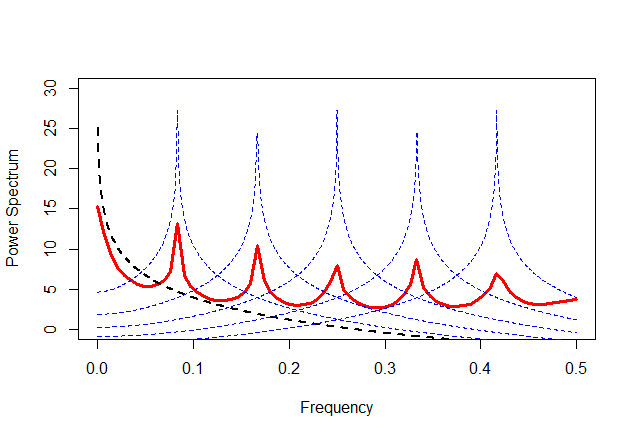
\includegraphics[scale = 0.40]{Plots/AR14airpass.png}
\caption{Red line: AR(14) fitted to the AirPassanger data. Black line: trend IRW component. Blue line: RW harmonic components. $\sigma^2$ is 1, whereas all the other $\sigma^2_{\omega_j}$ are 1/10. We plot the spectrum in log scale.}
\label{fig:AR14airpass}
\end{figure}

The code to realise this experiment is given as follows:

\begin{knitrout}\footnotesize
\definecolor{shadecolor}{rgb}{0.969, 0.969, 0.969}\color{fgcolor}\begin{kframe}
\begin{alltt}
\hlcom{####### Pseudo-spectra DHR model (AirPassengers Data)}
\hlkwd{library}\hlstd{(astsa)}
\hlkwd{data}\hlstd{(}\hlstr{"AirPassengers"}\hlstd{)}

\hlcom{# Variances: Obs variance, Trend variance, harmonic component variances}
\hlstd{sigma} \hlkwb{<-} \hlkwd{c}\hlstd{(}\hlnum{1}\hlstd{,} \hlnum{1}\hlopt{/}\hlnum{10}\hlstd{,} \hlkwd{rep}\hlstd{(}\hlnum{1}\hlopt{/}\hlnum{10}\hlstd{,} \hlnum{5}\hlstd{))}

\hlcom{# Trend frequency, Harmonic components frequencies}
\hlstd{omega.j} \hlkwb{<-} \hlkwd{c}\hlstd{(}\hlnum{0}\hlstd{,} \hlnum{1}\hlopt{/}\hlnum{12}\hlstd{,} \hlnum{1}\hlopt{/}\hlnum{6}\hlstd{,} \hlnum{1}\hlopt{/}\hlnum{4}\hlstd{,} \hlnum{1}\hlopt{/}\hlnum{3}\hlstd{,} \hlnum{1}\hlopt{/}\hlstd{(}\hlnum{2.4}\hlstd{))}


\hlcom{# Finding AR(p) to approximate spectrum of AirPassanger}
\hlkwd{performance.ar.p}\hlstd{(AirPassengers,} \hlkwc{p} \hlstd{=} \hlnum{20}\hlstd{,} \hlkwc{plot} \hlstd{=} \hlnum{TRUE}\hlstd{,} \hlkwc{legend} \hlstd{= F)}

\hlcom{# Fitting AR(14) to AirPassangers}
\hlstd{p} \hlkwb{<-} \hlnum{14}
\hlstd{fit} \hlkwb{<-} \hlkwd{arima}\hlstd{(AirPassengers,} \hlkwc{order} \hlstd{=} \hlkwd{c}\hlstd{(p,} \hlnum{0}\hlstd{,} \hlnum{0}\hlstd{),} \hlkwc{method}\hlstd{=}\hlstr{"ML"}\hlstd{)}
\hlstd{coef} \hlkwb{<-} \hlstd{fit}\hlopt{$}\hlstd{coef[}\hlnum{1}\hlopt{:}\hlstd{p]}

\hlcom{# Spectrum AR(14)}
\hlstd{ar.fit} \hlkwb{<-} \hlkwd{arma.spec}\hlstd{(}\hlkwc{ar} \hlstd{= coef,} \hlkwc{n.freq} \hlstd{=} \hlkwd{length}\hlstd{(freq)} \hlopt{+} \hlnum{1}\hlstd{,}
                    \hlkwc{var.noise} \hlstd{= fit}\hlopt{$}\hlstd{sigma2)}

\hlcom{# Plotting log(spectrum)}
\hlkwd{par}\hlstd{(}\hlkwc{mfrow} \hlstd{=} \hlkwd{c}\hlstd{(}\hlnum{1}\hlstd{,} \hlnum{1}\hlstd{))}
\hlkwd{plot}\hlstd{(ar.fit}\hlopt{$}\hlstd{freq,} \hlkwd{log}\hlstd{(ar.fit}\hlopt{$}\hlstd{spec),} \hlkwc{type} \hlstd{=} \hlstr{"l"}\hlstd{,} \hlkwc{col} \hlstd{=} \hlstr{"red"}\hlstd{,} \hlkwc{lwd} \hlstd{=} \hlnum{3}\hlstd{,}
     \hlkwc{xlab} \hlstd{=} \hlstr{"Frequency"}\hlstd{,} \hlkwc{ylab} \hlstd{=} \hlstr{"Power Spectrum"}\hlstd{,} \hlkwc{ylim} \hlstd{=} \hlkwd{c}\hlstd{(}\hlnum{0}\hlstd{,} \hlnum{30}\hlstd{))}

\hlcom{# Adding lines of the pseudo spectrum of IRW trend, and RW }
\hlcom{# harmonic components.}
\hlkwd{lines}\hlstd{(freq,} \hlkwd{log}\hlstd{(sigma[}\hlnum{2}\hlstd{]} \hlopt{*} \hlkwd{S}\hlstd{(freq, omega.j[}\hlnum{1}\hlstd{],} \hlkwc{type} \hlstd{=} \hlstr{"IRW"}\hlstd{)}\hlopt{/}\hlstd{(}\hlnum{2}\hlopt{*}\hlstd{pi)),}
      \hlkwc{lty} \hlstd{=} \hlnum{2}\hlstd{,} \hlkwc{lwd} \hlstd{=} \hlnum{2}\hlstd{)}
\hlkwa{for}\hlstd{(i} \hlkwa{in} \hlnum{2}\hlopt{:}\hlnum{6}\hlstd{) \{}
  \hlkwd{lines}\hlstd{(freq,} \hlkwd{log}\hlstd{(sigma[i} \hlopt{+} \hlnum{1}\hlstd{]} \hlopt{*} \hlkwd{S}\hlstd{(freq, omega.j[i],} \hlkwc{type} \hlstd{=} \hlstr{"IRW"}\hlstd{)}\hlopt{/}\hlstd{(}\hlnum{2}\hlopt{*}\hlstd{pi)),}
        \hlkwc{lty} \hlstd{=} \hlnum{2}\hlstd{,} \hlkwc{col} \hlstd{=} \hlstr{"blue"}\hlstd{)}
  \hlstd{\}}
\end{alltt}
\end{kframe}
\end{knitrout}


Then, the pseudo-spectrum of the full DHR model becomes:

\begin{equation}
\label{fullDHRmodel}
\boxed{
f_y(\omega, \underline{\sigma}^2) = \sum_{j = 0}^{R} \Big[ \sigma^2_{\omega_j}S(\omega, \omega_j) \Big] + \frac{\sigma^2}{2 \pi}
} \quad \text{where } \underline{\sigma}^2 = [\sigma^2, \sigma^2_{\omega_{0}}, \dots, \sigma^2_{\omega_{R}}]
\end{equation}


The code to compute the full DHR model with IRW trend, and RW harmonic components of \eqref{fullDHRmodel}


\begin{knitrout}\footnotesize
\definecolor{shadecolor}{rgb}{0.969, 0.969, 0.969}\color{fgcolor}\begin{kframe}
\begin{alltt}
\hlcom{###### Function to compute pseudo-spectrum full DHR (specific example)}

\hlcom{# sigma: vector of variances}
\hlcom{#        1st component is the observational variance}
\hlcom{#        2nd component is the trend variance}
\hlcom{#        3rd...Rth components are harmonic variances.}

\hlcom{# omega.j: vector of fondamental frequency and harmonics}
\hlcom{#          omega.j[1] must be 0 (if the trend is included)}

\hlstd{fullDHR.spectrum} \hlkwb{<-} \hlkwa{function}\hlstd{(}\hlkwc{omega}\hlstd{,} \hlkwc{sigma}\hlstd{,} \hlkwc{omega.j}\hlstd{) \{}

  \hlstd{R} \hlkwb{<-} \hlkwd{length}\hlstd{(omega.j)} \hlopt{-} \hlnum{1}

  \hlcom{# Trend component:}
  \hlstd{spectrum} \hlkwb{<-} \hlstd{sigma[}\hlnum{2}\hlstd{]} \hlopt{*} \hlkwd{S}\hlstd{(omega, omega.j[}\hlnum{1}\hlstd{],} \hlkwc{type} \hlstd{=} \hlstr{"IRW"}\hlstd{)}
  \hlkwd{print}\hlstd{(spectrum)}

  \hlcom{# Harmonic components:}
  \hlkwa{for}\hlstd{(j} \hlkwa{in} \hlnum{1}\hlopt{:}\hlstd{R) \{}
    \hlstd{spectrum} \hlkwb{=} \hlstd{spectrum} \hlopt{+} \hlstd{sigma[j} \hlopt{+} \hlnum{2}\hlstd{]} \hlopt{*} \hlkwd{S}\hlstd{(omega, omega.j[j} \hlopt{+} \hlnum{1}\hlstd{],} \hlkwc{type} \hlstd{=} \hlstr{"RW"}\hlstd{)}
  \hlstd{\}}

  \hlkwd{return}\hlstd{(spectrum} \hlopt{+} \hlstd{(sigma[}\hlnum{1}\hlstd{]}\hlopt{/}\hlstd{(}\hlnum{2}\hlopt{*}\hlstd{pi)))}
\hlstd{\}}
\end{alltt}
\end{kframe}
\end{knitrout}


\vspace{0.3cm}

\subsection*{Estimation in the Frequency Domain}

Equation \eqref{fullDHRmodel} can be considered as a linear combination of known spectral terms, with the unknown variance parameters appearing as regression coefficients.
To estimate $\underline{\sigma^2}$ we can minimise a cost function of the form

\begin{equation*}
E(\underline{\sigma}^2) = \sum_{i = 0}^{T - 1} \Big[ f_y(\omega_i) - \hat{f}_y(\omega_i,\underline{\sigma}^2) \Big]^2
\end{equation*}

where $f_y(\omega)$ is the empirical spectrum, for example the spectrum otbained by fitting an AR($p$) process to the data $y$. The $\omega_i$ are in the range 0 to 0.5, $i = 0, 1, 2, \dots, T - 1$.



An alternative error function, which is easier to minimise is the one defined on logarithmic terms:

\begin{equation*}
E(\underline{\sigma}^2)_{L} = \sum_{i = 0}^{T - 1} \Big[ \text{log}[f_y(\omega_i)] - \text{log}[\hat{f}_y(\omega_i,\underline{\sigma}^2)] \Big]^2
\end{equation*}

One final simplification is possible: if the empirical spectrum is defined on the estimated AR(p) spectrum, then $\sigma^2$, the estimate of the residual white noise can be used to get:


\begin{equation*}
f_y(\omega, \underline{NVR}) = \sigma^2 \Big[ \sum_{j = 0}^{R} \text{NVR}_j S(\omega, \omega_j) + \frac{1}{2 \pi} \Big],
\end{equation*}

where \textbf{NVR} is the vector with elements $NVR_j$ = $\dfrac{\sigma^2_{\omega_j}}{\sigma^2}$, $j = 0, 1, \dots, R$

\vspace{0.5cm}


\subsection*{The Complete DHR Estimation Algorithm }
In the case where a cyclical component is not present, the complete DHR algorithm can be expressed in four steps.

\subsubsection*{1. AR(p) spectrum estimation}
Estimate an AR(p) spectrum $f_y(\omega)$ and its associated residuals variance $\hat{\sigma}^2$, with the order $p$ identified by reference to AIC or BIC. In this way we can also choose the R frequency $\omega_j$ that drives the data.

The code for choosing p is given by:

\begin{knitrout}\footnotesize
\definecolor{shadecolor}{rgb}{0.969, 0.969, 0.969}\color{fgcolor}\begin{kframe}
\begin{alltt}
\hlstd{performance.ar.p} \hlkwb{<-} \hlkwa{function}\hlstd{(}\hlkwc{residuals.data}\hlstd{,} \hlkwc{p}\hlstd{,} \hlkwc{plot} \hlstd{=} \hlnum{TRUE}\hlstd{,} \hlkwc{legend} \hlstd{=} \hlnum{TRUE}\hlstd{) \{}

  \hlstd{T} \hlkwb{<-} \hlkwd{length}\hlstd{(residuals.data)}

  \hlstd{AIC} \hlkwb{<-} \hlkwd{rep}\hlstd{(}\hlnum{0}\hlstd{, p)}
  \hlstd{BIC} \hlkwb{<-} \hlkwd{rep}\hlstd{(}\hlnum{0}\hlstd{, p)}

  \hlkwa{for}\hlstd{(k} \hlkwa{in} \hlnum{1}\hlopt{:}\hlstd{p) \{}
    \hlstd{fit} \hlkwb{<-} \hlkwd{ar}\hlstd{(residuals.data,} \hlkwc{order} \hlstd{= k,} \hlkwc{aic} \hlstd{=} \hlnum{FALSE}\hlstd{)}
    \hlstd{sigma2} \hlkwb{<-} \hlkwd{var}\hlstd{(fit}\hlopt{$}\hlstd{resid,} \hlkwc{na.rm} \hlstd{=} \hlnum{TRUE}\hlstd{)}
    \hlstd{BIC[k]} \hlkwb{<-} \hlkwd{log}\hlstd{(sigma2)} \hlopt{+} \hlstd{(k}\hlopt{*}\hlkwd{log}\hlstd{(T)}\hlopt{/}\hlstd{T)}
    \hlstd{AIC[k]} \hlkwb{<-} \hlkwd{log}\hlstd{(sigma2)} \hlopt{+} \hlstd{((T}\hlopt{+}\hlnum{2}\hlopt{*}\hlstd{k)}\hlopt{/}\hlstd{T)}
  \hlstd{\}}

  \hlkwa{if} \hlstd{(plot} \hlopt{==} \hlnum{TRUE}\hlstd{) \{}
    \hlstd{IC} \hlkwb{<-} \hlkwd{cbind}\hlstd{(AIC, BIC)}
    \hlkwd{ts.plot}\hlstd{(IC,} \hlkwc{type} \hlstd{=} \hlstr{"o"}\hlstd{,} \hlkwc{xlab} \hlstd{=} \hlstr{"p"}\hlstd{,}
            \hlkwc{ylab} \hlstd{=} \hlstr{"AIC and BIC"}\hlstd{,} \hlkwc{col} \hlstd{=} \hlkwd{c}\hlstd{(}\hlstr{"red"}\hlstd{,} \hlstr{"blue"}\hlstd{),}
            \hlkwc{lwd} \hlstd{=} \hlnum{2}\hlstd{)}
    \hlkwd{points}\hlstd{(}\hlkwd{which}\hlstd{(BIC} \hlopt{==} \hlkwd{min}\hlstd{(BIC)), BIC[}\hlkwd{which}\hlstd{(BIC} \hlopt{==} \hlkwd{min}\hlstd{(BIC))],}
           \hlkwc{col} \hlstd{=} \hlstr{"black"}\hlstd{,} \hlkwc{pch} \hlstd{=} \hlnum{19}\hlstd{,} \hlkwc{lwd} \hlstd{=} \hlnum{4}\hlstd{)}
    \hlkwd{points}\hlstd{(}\hlkwd{which}\hlstd{(AIC} \hlopt{==} \hlkwd{min}\hlstd{(AIC)), AIC[}\hlkwd{which}\hlstd{(AIC} \hlopt{==} \hlkwd{min}\hlstd{(AIC))],}
           \hlkwc{col} \hlstd{=} \hlstr{"black"}\hlstd{,} \hlkwc{pch} \hlstd{=} \hlnum{19}\hlstd{,} \hlkwc{lwd} \hlstd{=} \hlnum{4}\hlstd{)}
    \hlkwa{if} \hlstd{(legend} \hlopt{==} \hlnum{TRUE}\hlstd{) \{}
    \hlkwd{legend}\hlstd{(}\hlstr{"bottomright"}\hlstd{,} \hlkwd{c}\hlstd{(}\hlstr{"AIC"}\hlstd{,} \hlstr{"BIC"}\hlstd{),} \hlkwc{lty} \hlstd{=} \hlnum{1}\hlstd{,} \hlkwc{lwd} \hlstd{=} \hlnum{2}\hlstd{,}
           \hlkwc{col} \hlstd{=} \hlkwd{c}\hlstd{(}\hlstr{"red"}\hlstd{,} \hlstr{"blue"}\hlstd{))}
    \hlstd{\}}
  \hlstd{\}}

  \hlkwd{return}\hlstd{(}\hlkwd{list}\hlstd{(}\hlkwc{AIC} \hlstd{= AIC,} \hlkwc{BIC} \hlstd{= BIC))}
\hlstd{\}}
\end{alltt}
\end{kframe}
\end{knitrout}

After having choosen $p$, the function to estimate the AR spectrum is given by below. 
This function requires as argoument the data to fit to an AR, the lag p, and the number of frequencies used. In order to avoid numerical problem, I decided to not consider frequency $\omega_i$ = 0. Indeed, given $T$ as number of frequency, this function will return the spectrum of (T-1) frequencies, the (T - 1) frequencies, and the estimated residual variance $\sigma^2$.


\begin{knitrout}\footnotesize
\definecolor{shadecolor}{rgb}{0.969, 0.969, 0.969}\color{fgcolor}\begin{kframe}
\begin{alltt}
\hlcom{#### Function Step 1: Estimate AR(p) spectrum of the observation process}
\hlkwd{require}\hlstd{(astsa)}
\hlstd{estimate.AR} \hlkwb{<-} \hlkwa{function}\hlstd{(}\hlkwc{data}\hlstd{,} \hlkwc{p}\hlstd{,} \hlkwc{n.freq}\hlstd{) \{}

  \hlcom{# Fitting AR(p) to data, getting the coefficients and the residual variance}
  \hlstd{fit} \hlkwb{<-} \hlkwd{arima}\hlstd{(data,} \hlkwc{order} \hlstd{=} \hlkwd{c}\hlstd{(p,} \hlnum{0}\hlstd{,} \hlnum{0}\hlstd{),} \hlkwc{method} \hlstd{=} \hlstr{"ML"}\hlstd{)}
  \hlstd{coef} \hlkwb{<-} \hlstd{fit}\hlopt{$}\hlstd{coef[}\hlnum{1}\hlopt{:}\hlstd{p]}
  \hlstd{sigma2} \hlkwb{<-} \hlstd{fit}\hlopt{$}\hlstd{sigma2}

  \hlcom{# Getting spectrum AR(p)}
  \hlstd{ar.fit} \hlkwb{<-} \hlkwd{arma.spec}\hlstd{(}\hlkwc{ar} \hlstd{= coef,} \hlkwc{n.freq} \hlstd{= n.freq,} \hlkwc{var.noise} \hlstd{= fit}\hlopt{$}\hlstd{sigma2)}

  \hlcom{# Not considering frequency 0}
  \hlstd{spectrum} \hlkwb{<-} \hlstd{ar.fit}\hlopt{$}\hlstd{spec[}\hlopt{-}\hlnum{1}\hlstd{]}
  \hlstd{freq} \hlkwb{<-} \hlstd{ar.fit}\hlopt{$}\hlstd{freq[}\hlopt{-}\hlnum{1}\hlstd{]}

  \hlkwd{return}\hlstd{(}\hlkwd{list}\hlstd{(}\hlkwc{spectrum} \hlstd{= spectrum,} \hlkwc{frequency} \hlstd{= freq ,} \hlkwc{sigma2} \hlstd{= sigma2))}
\hlstd{\}}
\end{alltt}
\end{kframe}
\end{knitrout}


\vspace{0.2cm}

\subsubsection*{2. Linear Least Square estimate of the NVR parameters}
Let \textbf{$\mathbf{Y}$} be the vector with components 
\begin{equation*}
y_i = f_y(\omega_i) - \frac{\sigma^2}{2\pi}, \quad i = 1,\dots, T - 1
\end{equation*}
Let \textbf{X} be the matrix, with elements:
\begin{equation*}
x_{ij} = \sigma^2  S(\omega_i, \omega_j), \quad j = 1, \dots, R
\end{equation*}

In this way \textbf{Y} = \textbf{X}$\cdot$\textbf{NVR} + $\epsilon$, and the linear least square estimate of $NVR$ is given by:


\begin{equation*}
\widehat{\mathbf{NVR}} = (\mathbf{X}^t \mathbf{X})^{-1} \mathbf{X}^t \mathbf{Y}
\end{equation*}

The code for performing this step is given below. This function will return the $NVR$ estimates.

\begin{knitrout}\footnotesize
\definecolor{shadecolor}{rgb}{0.969, 0.969, 0.969}\color{fgcolor}\begin{kframe}
\begin{alltt}
\hlcom{#### Function Step 2: Find Linear Least Square estimate of NVR parameter vector}

\hlstd{NVR.LinearLS} \hlkwb{<-} \hlkwa{function}\hlstd{(}\hlkwc{empirical.spectrum}\hlstd{,} \hlkwc{sigma2}\hlstd{,}
                         \hlkwc{frequency}\hlstd{,} \hlkwc{omega.j}\hlstd{,} \hlkwc{structures}\hlstd{) \{}

  \hlcom{# Number of frequencies}
  \hlstd{T} \hlkwb{<-} \hlkwd{length}\hlstd{(frequency)}
  \hlcom{# Number of harmonic components}
  \hlstd{R} \hlkwb{<-} \hlkwd{length}\hlstd{(omega.j)} \hlopt{-} \hlnum{1}

  \hlcom{# Preparing data for evaluating LLS NVR estimate}
  \hlstd{Y} \hlkwb{<-} \hlstd{empirical.spectrum} \hlopt{-} \hlstd{(sigma2}\hlopt{/}\hlstd{(}\hlnum{2}\hlopt{*}\hlstd{pi))}
  \hlstd{X} \hlkwb{<-} \hlkwd{matrix}\hlstd{(}\hlnum{NA}\hlstd{,} \hlkwc{nrow} \hlstd{= T,} \hlkwc{ncol} \hlstd{= (R} \hlopt{+} \hlnum{1}\hlstd{))}

  \hlkwa{for}\hlstd{(r} \hlkwa{in} \hlnum{1}\hlopt{:}\hlstd{(R} \hlopt{+} \hlnum{1}\hlstd{)) \{}
    \hlstd{X[, r]} \hlkwb{<-} \hlkwd{S}\hlstd{(frequency, omega.j[r],} \hlkwc{type} \hlstd{= structures[r])}
  \hlstd{\}}

  \hlstd{X} \hlkwb{<-} \hlstd{sigma2} \hlopt{*} \hlstd{X}

  \hlcom{# Least square estimate}
  \hlstd{NVR.estimate} \hlkwb{<-} \hlkwd{solve}\hlstd{(}\hlkwd{t}\hlstd{(X)} \hlopt \hlstd{X,} \hlkwd{t}\hlstd{(X)} \hlopt \hlstd{Y)}

  \hlkwd{return}\hlstd{(NVR.estimate)}
\hlstd{\}}
\end{alltt}
\end{kframe}
\end{knitrout}
\vspace{0.2cm}
\textit{Testing Step 2}

I am not sure if the results are correct, because I get different numbers from the paper. But it looks to me that the code, and the procedure is right.
To see indeed if the results that I got are reasonable, I evaluated and plotted the DHR spectrum, with the estimated $\hat{\underline{\sigma}}^2$. 
In Figure \ref{fig:firstestimateDHR} we show the true AR(14) spectrum fitted to the \texttt{AirPassangers} Data with the red line; the green line is the spectrum given by \eqref{fullDHRmodel}, with $\hat{\underline{\sigma}}^2$ estimated by LLS. The results look sensible.



\begin{knitrout}\footnotesize
\definecolor{shadecolor}{rgb}{0.969, 0.969, 0.969}\color{fgcolor}\begin{kframe}
\begin{alltt}
\hlcom{# Testing steps of Complete DHR Estimation Algorithm }

\hlcom{# Getting data}
\hlstd{data.AP} \hlkwb{<-} \hlstd{AirPassengers}
\hlcom{# Harmonics}
\hlstd{omega.j.AP} \hlkwb{<-} \hlkwd{c}\hlstd{(}\hlnum{0}\hlstd{,} \hlnum{1}\hlopt{/}\hlnum{12}\hlstd{,} \hlnum{1}\hlopt{/}\hlnum{6}\hlstd{,} \hlnum{1}\hlopt{/}\hlnum{4}\hlstd{,} \hlnum{1}\hlopt{/}\hlnum{3}\hlstd{,} \hlnum{1}\hlopt{/}\hlstd{(}\hlnum{2.4}\hlstd{))}
\hlcom{# IRW Trend, RW harmonic components}
\hlstd{structures.AP} \hlkwb{<-} \hlkwd{c}\hlstd{(}\hlstr{"IRW"}\hlstd{,} \hlkwd{rep}\hlstd{(}\hlstr{"RW"}\hlstd{,} \hlnum{5}\hlstd{))}

\hlcom{# Getting spectrum and residuals variance from AR(P) fitted to AirPassengers}
\hlstd{AP.AR14} \hlkwb{<-} \hlkwd{estimate.AR}\hlstd{(}\hlkwc{data} \hlstd{= data.AP,} \hlkwc{p} \hlstd{=} \hlnum{14}\hlstd{,} \hlkwc{n.freq} \hlstd{=} \hlkwd{length}\hlstd{(data.AP))}
\hlstd{freq} \hlkwb{<-} \hlstd{AP.AR14}\hlopt{$}\hlstd{frequency}
\hlstd{spec} \hlkwb{<-} \hlstd{AP.AR14}\hlopt{$}\hlstd{spectrum}
\hlstd{sigma2} \hlkwb{<-} \hlstd{AP.AR14}\hlopt{$}\hlstd{sigma2}

\hlcom{# Estimating NVR with Step2 (LLS)}
\hlstd{NVR.LSS.estimate} \hlkwb{<-} \hlkwd{NVR.LinearLS}\hlstd{(}\hlkwc{empirical.spectrum} \hlstd{= spec,}
                                 \hlkwc{sigma2} \hlstd{= sigma2,}
                                 \hlkwc{frequency} \hlstd{= frequency,}
                                 \hlkwc{omega.j} \hlstd{= omega.j.AP,}
                                 \hlkwc{structures} \hlstd{= structures.AP)}

\hlcom{# Sigma estimate}
\hlstd{sigma.est} \hlkwb{<-} \hlkwd{c}\hlstd{(sigma2, sigma2} \hlopt{*} \hlstd{NVR.LSS.estimate)}

\hlcom{# Plotting AR(14) spectrum and DHR spectrum with estimated sigma (LLS)}
\hlkwd{plot}\hlstd{(freq,} \hlkwd{log}\hlstd{(spec),} \hlkwc{type} \hlstd{=} \hlstr{"l"}\hlstd{,} \hlkwc{col} \hlstd{=} \hlstr{"red"}\hlstd{,} \hlkwc{lwd} \hlstd{=} \hlnum{2}\hlstd{)}
\hlkwd{lines}\hlstd{(freq,} \hlkwd{log}\hlstd{(}\hlkwd{fullDHR.spectrum}\hlstd{(freq,  sigma.est, omega.j.AP)),}
      \hlkwc{lwd} \hlstd{=} \hlnum{2}\hlstd{,} \hlkwc{col} \hlstd{=} \hlstr{"green"}\hlstd{)}
\end{alltt}
\end{kframe}
\end{knitrout}

\begin{figure}[htbp]
\centering
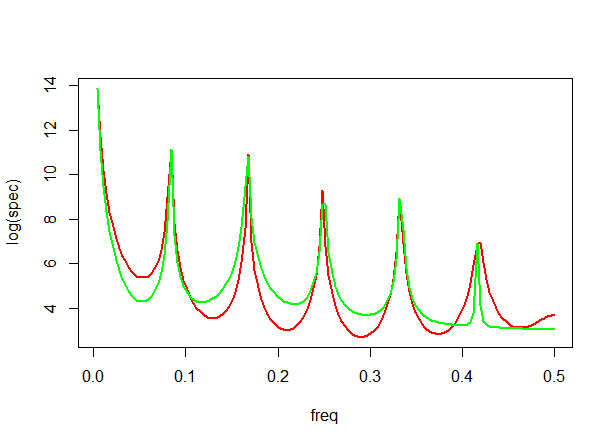
\includegraphics[scale = 0.4]{Plots/firstestimateDHR.png}
\caption{Red line: AR(14) spectrum for \texttt{AirPassangers}. Green line: full DHR spectrum with estimated variances from Step 2.}
\label{fig:firstestimateDHR}
\end{figure}


\subsubsection*{3. Optimisation of Logaritmich Loss}
In this step the we optimise 

\begin{equation*}
E(\mathbf{NVR})_{L} = \sum_{i = 0}^{T - 1} \Big[ \text{log}[f_y(\omega_i)] - \text{log}[\hat{f}_y(\omega_i, NVR)] \Big]^2,
\end{equation*}
using as initial conditions the values of $\widehat{\mathbf{NVR}}$ obtained in Step 2.

We give below the code to implement the logarithmic loss function, and we show that the estimate of this non linear function, has improved the fitting to the AR(14) spectrum. 

\begin{knitrout}\footnotesize
\definecolor{shadecolor}{rgb}{0.969, 0.969, 0.969}\color{fgcolor}\begin{kframe}
\begin{alltt}
\hlcom{#### Function Step 3:  evaluate the logarithmic error.}

\hlstd{E} \hlkwb{<-} \hlkwa{function}\hlstd{(}\hlkwc{NVR}\hlstd{,} \hlkwc{freq}\hlstd{,} \hlkwc{empirical.spectrum}\hlstd{,} \hlkwc{omega.j}\hlstd{,} \hlkwc{structures}\hlstd{,} \hlkwc{sigma2}\hlstd{) \{}


  \hlcom{# Number of frequencies}
  \hlstd{T} \hlkwb{<-} \hlkwd{length}\hlstd{(freq)}
  \hlcom{# Number of harmonic components}
  \hlstd{R} \hlkwb{<-} \hlkwd{length}\hlstd{(omega.j)} \hlopt{-} \hlnum{1}

  \hlcom{# Matrix T * (R + 1) with components X[i, j] <- S(omega_i, omega_j)}
  \hlstd{X} \hlkwb{<-} \hlkwd{matrix}\hlstd{(}\hlnum{NA}\hlstd{,} \hlkwc{nrow} \hlstd{= T,} \hlkwc{ncol} \hlstd{= (R} \hlopt{+} \hlnum{1}\hlstd{))}
  \hlkwa{for}\hlstd{(r} \hlkwa{in} \hlnum{1}\hlopt{:}\hlstd{(R} \hlopt{+} \hlnum{1}\hlstd{)) \{}
    \hlstd{X[, r]} \hlkwb{<-} \hlkwd{S}\hlstd{(freq, omega.j[r],} \hlkwc{type} \hlstd{= structures[r])}
  \hlstd{\}}

  \hlstd{fitted} \hlkwb{<-} \hlstd{sigma2} \hlopt{*} \hlstd{((X} \hlopt \hlstd{NVR)} \hlopt{+} \hlstd{(}\hlnum{1}\hlopt{/}\hlstd{(}\hlnum{2}\hlopt{*}\hlstd{pi)))}

  \hlcom{# Evaluating E(sigma)_L; }
  \hlstd{error} \hlkwb{<-} \hlkwd{sum}\hlstd{((}\hlkwd{log}\hlstd{(empirical.spectrum)} \hlopt{-}
                  \hlkwd{log}\hlstd{(fitted))}\hlopt{^}\hlnum{2}\hlstd{)}

  \hlkwd{return}\hlstd{(error)}
\hlstd{\}}
\end{alltt}
\end{kframe}
\end{knitrout}

\vspace{0.2cm}
\textit{Testing Step 3 - Optimisation of Logaritmich Loss}

We optimise the error function given above, by using \texttt{optim}.

We obtained some warnings, like \texttt{In log(fitted) : NaNs produced}. But the results is reassuring, given that the paper doesn't seems to do better.
\begin{knitrout}\footnotesize
\definecolor{shadecolor}{rgb}{0.969, 0.969, 0.969}\color{fgcolor}\begin{kframe}
\begin{alltt}
\hlcom{# Optimising logarithmic error: (THERE ARE WARNINGS)}
\hlstd{optimising.NVR} \hlkwb{<-} \hlkwd{optim}\hlstd{(NVR.LSS.estimate, E,}
                        \hlkwc{freq} \hlstd{= freq,} \hlkwc{empirical.spectrum} \hlstd{= spec,}
                        \hlkwc{omega.j} \hlstd{= omega.j.AP,} \hlkwc{structures} \hlstd{= structures.AP,}
                        \hlkwc{sigma2} \hlstd{= sigma2,} \hlkwc{method} \hlstd{=} \hlstr{"Nelder-Mead"}\hlstd{)}

\hlcom{# Final NVR estimate}
\hlstd{NVR.nonlinear.estimate} \hlkwb{<-} \hlstd{optimising.NVR}\hlopt{$}\hlstd{par}

\hlcom{# Final sigma^2 estimate}
\hlstd{final.sigma.est} \hlkwb{<-} \hlkwd{c}\hlstd{(sigma2, sigma2} \hlopt{*} \hlstd{NVR.nonlinear.estimate)}

\hlcom{# Plotting AR(14) spectrum and DHR spectrum with estimated sigma, }
\hlcom{# by using log loss function}

\hlkwd{plot}\hlstd{(freq,} \hlkwd{log}\hlstd{(spec),} \hlkwc{type} \hlstd{=} \hlstr{"l"}\hlstd{,} \hlkwc{col} \hlstd{=} \hlstr{"red"}\hlstd{,} \hlkwc{lwd} \hlstd{=} \hlnum{2}\hlstd{)}
\hlkwd{lines}\hlstd{(freq,} \hlkwd{log}\hlstd{(}\hlkwd{fullDHR.spectrum}\hlstd{(freq,  final.sigma.est, omega.j.AP)),}
      \hlkwc{lwd} \hlstd{=} \hlnum{2}\hlstd{,} \hlkwc{col} \hlstd{=} \hlstr{"green"}\hlstd{)}
\end{alltt}
\end{kframe}
\end{knitrout}


\begin{figure}[htbp]
\centering
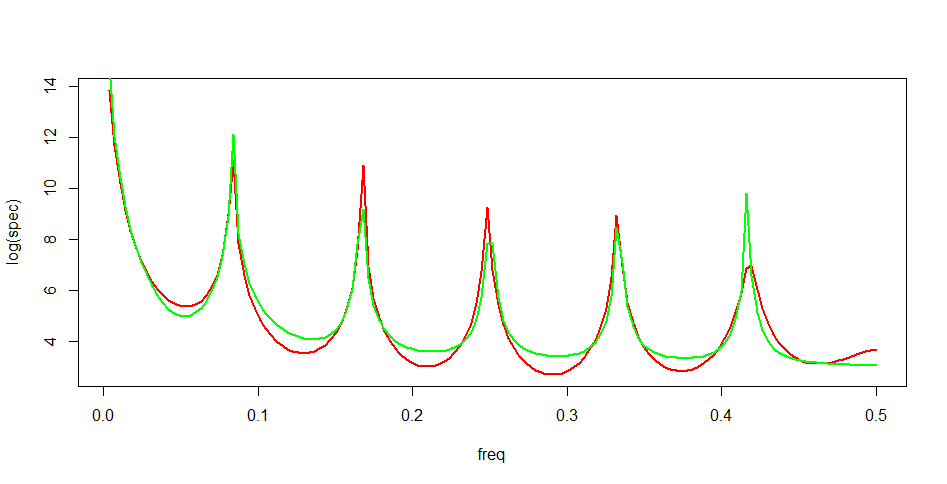
\includegraphics[scale = 0.4]{Plots/finalNVRestimateAR14}
\caption{Red line: AR(14) spectrum for \texttt{AirPassangers}. Green line: full DHR spectrum with estimated variances from Step 3}
\end{figure}

\newpage

\subsubsection*{4. Kalman Filter and Smoothing}
This step consists on the filtering and the smoothing techniques described at the beginning of the paper. 

\vspace{0.3cm}

\textbf{Filtering}

Let be R be the number of harmonic components used, and let $n = 2(R + 1)$

The arguments for the Kalman Filter function are

\begin{itemize}
\item \texttt{y}, the observed time series
\item \texttt{F}, the system matrix. It's a block diagonal n$\times$n matrix, where each 2$\times$2 sub matrix is of the form:
\[ F_r = 
\begin{bmatrix} \alpha & \beta    \\ 0 & \gamma   \end{bmatrix}, \quad r = 0, 1, \dots, R.
\]

For \textbf{IRW}, we have $\alpha = \beta = \gamma = 1$. For \textbf{RW}, we have $\alpha = \gamma = 1$ and $\beta = 0$.

\item \texttt{H}, the observational matrix. It's a $ 1 \times n$ matrix. It basically describes the DHR model. It has to be a list of $T$ matrixes, where $$
H_t = [ \text{cos}(t \omega_0), \text{sin}(t \omega_0), \dots, \text{cos}(t \omega_R), \text{sin}(t \omega_R)] $$

\item \texttt{G}, the covariance matrix that control the system noise. It's a $n\times n$ matrix block diagonal matrix, with components:

\[ G_r = 
\begin{bmatrix} \delta & 0    \\ 0 & 1   \end{bmatrix}, \quad r = 0, 1, \dots, R.
\]

For \textbf{IRW}, we have $\delta = 0$. For \textbf{RW}, we have $\delta = 1$



\item \texttt{Q}, the covariance matrix of the system noise. It's a $n \times n$ diagonal matrix, with diagonal components:

$$ [\sigma^2_{\omega_0}, \sigma^2_{\omega_0},\dots, \sigma^2_{\omega_R}, \sigma^2_{\omega_R} ] $$

\item \texttt{sigma2} is $\sigma^2$, the observational variance, estimated in Step 1, from the AR(p) fitting.  

\end{itemize}

\vspace{0.5cm}

The code to perform the Kalman Filter, and some auxiliary functions are given below. The function \texttt{Kalman.Filter} return an object of class \texttt{Kalman.Filter} which is a list with several elements, for which the most relevant ones are 
\begin{itemize}

\item \texttt{states}, a list of filtered states $\mathbf{x}_t$, for $t = 1, \dots, T$.

\item \texttt{covariance.states}, a list of filtered (scaled) covariance matrixes $\dfrac{P_t}{\sigma^2}$,  for $t = 1, \dots, T$.
\end{itemize}

Other objects are returned from this function, which we'll be useful for the smoothing. 
\begin{knitrout}\footnotesize
\definecolor{shadecolor}{rgb}{0.969, 0.969, 0.969}\color{fgcolor}\begin{kframe}
\begin{alltt}
\hlcom{####### Kalman Filter:  Forward Pass Filtering #########}

\hlkwd{require}\hlstd{(Matrix)}
\hlcom{# Function to implement Forward Pass Filtering Equations (Kalman)}

\hlstd{Kalman.Filter} \hlkwb{<-} \hlkwa{function}\hlstd{(}\hlkwc{y}\hlstd{,} \hlkwc{F}\hlstd{,} \hlkwc{H}\hlstd{,} \hlkwc{G}\hlstd{,} \hlkwc{Q}\hlstd{,} \hlkwc{sigma2}\hlstd{) \{}

  \hlcom{# Length of the time series}
  \hlstd{T} \hlkwb{<-} \hlkwd{length}\hlstd{(y)}

  \hlcom{# Number of states  [(Trend + N.Harmonics) * 2]}
  \hlstd{n} \hlkwb{<-} \hlkwd{length}\hlstd{(omega.j)} \hlopt{*} \hlnum{2}


  \hlcom{# Checking dimensionality}
  \hlkwa{if}\hlstd{(}\hlopt{!}\hlstd{(} \hlkwd{all}\hlstd{(}\hlkwd{dim}\hlstd{(F)} \hlopt{==} \hlkwd{c}\hlstd{(n, n))} \hlopt{&} \hlkwd{all}\hlstd{(}\hlkwd{dim}\hlstd{(G)} \hlopt{==} \hlkwd{c}\hlstd{(n, n))} \hlopt{&}
        \hlkwd{all}\hlstd{(}\hlkwd{dim}\hlstd{(Q)} \hlopt{==} \hlkwd{c}\hlstd{(n, n))} \hlopt{&} \hlkwd{all}\hlstd{(}\hlkwd{dim}\hlstd{(H[[T]])} \hlopt{==} \hlkwd{c}\hlstd{(}\hlnum{1}\hlstd{, n)))) \{}
    \hlkwd{stop}\hlstd{(}\hlstr{"Matrix dimensions are incorrect"}\hlstd{)}
  \hlstd{\}}

  \hlcom{# States}
  \hlstd{states} \hlkwb{<-} \hlkwd{list}\hlstd{()}
  \hlstd{states[[}\hlnum{1}\hlstd{]]} \hlkwb{<-} \hlkwd{matrix}\hlstd{(}\hlkwd{rep}\hlstd{(}\hlnum{0}\hlstd{, n),} \hlkwc{nrow} \hlstd{= n,} \hlkwc{ncol} \hlstd{=} \hlnum{1}\hlstd{)}

  \hlcom{# Covariances matrix}
  \hlstd{covariance.states} \hlkwb{<-} \hlkwd{list}\hlstd{()}
  \hlstd{covariance.states[[}\hlnum{1}\hlstd{]]} \hlkwb{<-} \hlkwd{diag}\hlstd{(n)}

  \hlcom{# Q.r: matrix containing (scaled) system noise }
  \hlstd{Q.r} \hlkwb{<-} \hlstd{Q} \hlopt{/} \hlstd{sigma2}

  \hlcom{# Intermediate calculation steps}
  \hlstd{prediction.x} \hlkwb{<-} \hlkwd{list}\hlstd{()}
  \hlstd{prediction.P} \hlkwb{<-} \hlkwd{list}\hlstd{()}


  \hlcom{### Forward Pass Filtering Equations ###}

  \hlkwa{for}\hlstd{(t} \hlkwa{in} \hlnum{2}\hlopt{:}\hlstd{T) \{}
    \hlcom{# Prediction}
    \hlstd{prediction.x[[t]]} \hlkwb{<-} \hlstd{F} \hlopt \hlstd{states[[t} \hlopt{-} \hlnum{1}\hlstd{]]}

    \hlstd{prediction.P[[t]]} \hlkwb{<-} \hlstd{F} \hlopt \hlstd{covariance.states[[t} \hlopt{-} \hlnum{1}\hlstd{]]} \hlopt \hlkwd{t}\hlstd{(F)} \hlopt{+}
      \hlstd{G} \hlopt \hlstd{Q.r} \hlopt \hlkwd{t}\hlstd{(G)}

    \hlcom{# Correction}
    \hlstd{states[[t]]} \hlkwb{<-} \hlstd{prediction.x[[t]]} \hlopt{+} \hlstd{prediction.P[[t]]} \hlopt \hlkwd{t}\hlstd{(H[[t]])} \hlopt
      \hlkwd{solve}\hlstd{(}\hlnum{1} \hlopt{+} \hlstd{H[[t]]} \hlopt \hlstd{prediction.P[[t]]} \hlopt \hlkwd{t}\hlstd{(H[[t]]),}
            \hlstd{y[t]} \hlopt{-} \hlstd{H[[t]]} \hlopt \hlstd{prediction.x[[t]])}

    \hlstd{covariance.states[[t]]} \hlkwb{<-} \hlstd{prediction.P[[t]]} \hlopt{-} \hlstd{prediction.P[[t]]} \hlopt \hlkwd{t}\hlstd{(H[[t]])} \hlopt
      \hlkwd{solve}\hlstd{(}\hlnum{1} \hlopt{+} \hlstd{H[[t]]} \hlopt \hlstd{prediction.P[[t]]} \hlopt \hlkwd{t}\hlstd{(H[[t]]),}
            \hlstd{H[[t]]} \hlopt \hlstd{prediction.P[[t]])}
  \hlstd{\}}

  \hlstd{filtered.process} \hlkwb{<-} \hlkwd{list}\hlstd{(}\hlkwc{states} \hlstd{= states,}
                           \hlkwc{covariance.states} \hlstd{= covariance.states,}
                           \hlkwc{prediction.x} \hlstd{= prediction.x,}
                           \hlkwc{prediction.P} \hlstd{= prediction.P,}
                           \hlkwc{y} \hlstd{= y,} \hlkwc{F} \hlstd{= F,} \hlkwc{H} \hlstd{= H,}
                           \hlkwc{G} \hlstd{= G,} \hlkwc{Q} \hlstd{= Q,} \hlkwc{sigma2} \hlstd{= sigma2)}

  \hlkwd{class}\hlstd{(filtered.process)} \hlkwb{<-} \hlstr{"Kalman.Filter"}

  \hlkwd{return}\hlstd{(filtered.process)}
\hlstd{\}}
\end{alltt}
\end{kframe}
\end{knitrout}



\begin{knitrout}\footnotesize
\definecolor{shadecolor}{rgb}{0.969, 0.969, 0.969}\color{fgcolor}\begin{kframe}
\begin{alltt}
\hlcom{# Function to compute the fitted value of y, given the states,}
\hlcom{# and the model. }

\hlstd{fitted.DHR} \hlkwb{<-} \hlkwa{function}\hlstd{(}\hlkwc{H}\hlstd{,} \hlkwc{states}\hlstd{) \{}
  \hlstd{T} \hlkwb{<-} \hlkwd{length}\hlstd{(H)}
  \hlstd{fitted} \hlkwb{<-} \hlkwd{c}\hlstd{()}
  \hlkwa{for}\hlstd{(t} \hlkwa{in} \hlnum{1}\hlopt{:}\hlstd{T) \{}
    \hlstd{fitted[t]} \hlkwb{<-} \hlkwd{as.numeric}\hlstd{(H[[t]]} \hlopt \hlstd{states[[t]])}
  \hlstd{\}}
  \hlkwd{return}\hlstd{(fitted)}
\hlstd{\}}

\hlcom{# Function to create the time variable vector H}
\hlstd{get.H} \hlkwb{<-} \hlkwa{function}\hlstd{(}\hlkwc{omega.j}\hlstd{,} \hlkwc{T}\hlstd{) \{}
  \hlstd{H} \hlkwb{<-} \hlkwd{list}\hlstd{()}
  \hlkwa{for}\hlstd{(t} \hlkwa{in} \hlnum{1}\hlopt{:}\hlstd{T) \{}
    \hlstd{H[[t]]} \hlkwb{<-} \hlkwd{matrix}\hlstd{(}\hlkwd{c}\hlstd{(}\hlkwd{rbind}\hlstd{(}\hlkwd{cos}\hlstd{(omega.j} \hlopt{*} \hlstd{t),} \hlkwd{sin}\hlstd{(omega.j} \hlopt{*} \hlstd{t))),} \hlkwc{nrow} \hlstd{=} \hlnum{1}\hlstd{)}
  \hlstd{\}}
  \hlkwd{return}\hlstd{(H)}
\hlstd{\}}
\end{alltt}
\end{kframe}
\end{knitrout}


\vspace{0.2cm}
\textit{Testing Step 4 - Filtering}
\begin{knitrout}\footnotesize
\definecolor{shadecolor}{rgb}{0.969, 0.969, 0.969}\color{fgcolor}\begin{kframe}
\begin{alltt}
\hlcom{####### Preparing system, and observational matrixes #####}
\hlstd{R} \hlkwb{<-} \hlnum{1} \hlopt{+} \hlnum{5} \hlcom{# Trend + Harmonic TVP's}
\hlstd{n} \hlkwb{<-} \hlnum{2}\hlopt{*}\hlstd{R}
\hlstd{omega.j} \hlkwb{<-} \hlkwd{c}\hlstd{(}\hlnum{0}\hlstd{,} \hlnum{1}\hlopt{/}\hlnum{12}\hlstd{,} \hlnum{1}\hlopt{/}\hlnum{6}\hlstd{,} \hlnum{1}\hlopt{/}\hlnum{4}\hlstd{,} \hlnum{1}\hlopt{/}\hlnum{3}\hlstd{,} \hlnum{1}\hlopt{/}\hlstd{(}\hlnum{2.4}\hlstd{))}

\hlcom{# Matrix H}
\hlstd{H} \hlkwb{<-} \hlkwd{get.H}\hlstd{(omega.j, T)}

\hlcom{# Matrix F}
\hlstd{F.IRW} \hlkwb{<-} \hlkwd{matrix}\hlstd{(}\hlkwd{c}\hlstd{(}\hlnum{1}\hlstd{,} \hlnum{0}\hlstd{,} \hlnum{1}\hlstd{,} \hlnum{1}\hlstd{),} \hlkwc{nrow} \hlstd{=} \hlnum{2}\hlstd{,} \hlkwc{ncol} \hlstd{=} \hlnum{2}\hlstd{)}
\hlstd{F.RW} \hlkwb{<-} \hlkwd{matrix}\hlstd{(}\hlkwd{c}\hlstd{(}\hlnum{1}\hlstd{,} \hlnum{0}\hlstd{,} \hlnum{0}\hlstd{,} \hlnum{1}\hlstd{),} \hlkwc{nrow} \hlstd{=} \hlnum{2}\hlstd{,} \hlkwc{ncol} \hlstd{=} \hlnum{2}\hlstd{)}
\hlstd{F} \hlkwb{<-} \hlkwd{bdiag}\hlstd{(}\hlkwd{c}\hlstd{(}\hlkwd{list}\hlstd{(F.IRW),} \hlkwd{replicate}\hlstd{((R} \hlopt{-} \hlnum{1}\hlstd{), F.RW,} \hlkwc{simplify} \hlstd{=} \hlnum{FALSE}\hlstd{)))}

\hlcom{# Matrix G}
\hlstd{G.IRW} \hlkwb{<-} \hlkwd{matrix}\hlstd{(}\hlkwd{c}\hlstd{(}\hlnum{0}\hlstd{,} \hlnum{0}\hlstd{,} \hlnum{0}\hlstd{,} \hlnum{1}\hlstd{),} \hlkwc{nrow} \hlstd{=} \hlnum{2}\hlstd{,} \hlkwc{ncol} \hlstd{=} \hlnum{2}\hlstd{)}
\hlstd{G.RW} \hlkwb{<-} \hlkwd{matrix}\hlstd{(}\hlkwd{c}\hlstd{(}\hlnum{1}\hlstd{,} \hlnum{0}\hlstd{,} \hlnum{0}\hlstd{,} \hlnum{1}\hlstd{),} \hlkwc{nrow} \hlstd{=} \hlnum{2}\hlstd{,} \hlkwc{ncol} \hlstd{=} \hlnum{2}\hlstd{)}
\hlstd{G} \hlkwb{<-} \hlkwd{bdiag}\hlstd{(}\hlkwd{c}\hlstd{(}\hlkwd{list}\hlstd{(G.IRW),} \hlkwd{replicate}\hlstd{((R} \hlopt{-} \hlnum{1}\hlstd{), G.RW,} \hlkwc{simplify} \hlstd{=} \hlnum{FALSE}\hlstd{)))}

\hlcom{# Matrix Q}
\hlstd{Q} \hlkwb{<-} \hlkwd{diag}\hlstd{(}\hlkwd{rep}\hlstd{(sigma2} \hlopt{*} \hlstd{NVR.LSS.estimate,} \hlnum{1}\hlstd{,} \hlkwc{each} \hlstd{=} \hlnum{2}\hlstd{))}



\hlcom{#### Filtering:}
\hlstd{filtered.process} \hlkwb{<-} \hlkwd{Kalman.Filter}\hlstd{(}\hlkwc{y} \hlstd{= data.AP,} \hlkwc{F} \hlstd{= F,} \hlkwc{H} \hlstd{= H,} \hlkwc{G} \hlstd{= G,}
                                  \hlkwc{Q} \hlstd{= Q,} \hlkwc{sigma2} \hlstd{= sigma2)}

\hlstd{states} \hlkwb{<-} \hlstd{filtered.process}\hlopt{$}\hlstd{states}
\hlstd{covariance.states} \hlkwb{<-} \hlstd{filtered.process}\hlopt{$}\hlstd{covariance.states}

\hlcom{# Fitted values}
\hlstd{fitted} \hlkwb{<-} \hlkwd{fitted.DHR}\hlstd{(H, states)}

\hlcom{# Plotting true and fitted value (after Filtering)}
\hlkwd{plot}\hlstd{(}\hlnum{1}\hlopt{:}\hlstd{t, data.AP,} \hlkwc{type} \hlstd{=} \hlstr{"o"}\hlstd{)}
\hlkwd{lines}\hlstd{(}\hlnum{1}\hlopt{:}\hlstd{t, fitted,} \hlkwc{type} \hlstd{=} \hlstr{"o"}\hlstd{,} \hlkwc{col} \hlstd{=} \hlstr{"red"}\hlstd{)}
\end{alltt}
\end{kframe}
\end{knitrout}

\begin{figure}[htbp]
\centering
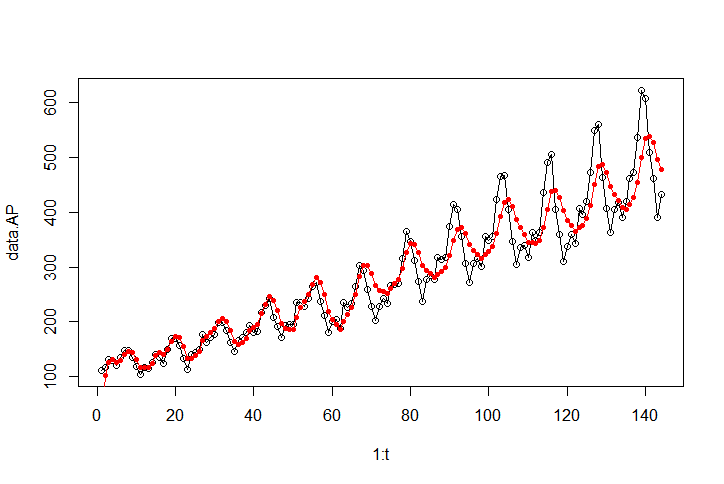
\includegraphics[scale = 0.5]{Plots/filteringpass.png}
\caption{Filtered fitted values to the \texttt{AirPassangers} data}
\end{figure}



\end{document}
